\title{System Dynamics:  Exercise 3 - Adaptation in Chemotaxis}
\author{Ryan Spangler}
\date{\today}

\documentclass[12pt]{article}

\usepackage{graphicx}

\begin{document}
\maketitle

\section{Approach}

For this exercise I chose to make a simple model of biological adaptation.  Adaptation is a word that is used in many ways throughout many fields, but in this particular case I am referring to it in the way that \cite{Alon} defines it, that a particular quality of a system returns to a set point after a perturbation, compensating for the perturbation with respect to whatever quality is being described.  In the case of this exercise I am choosing the subject to be the biological circuit involved in bacterial chemotaxis.   (Most of the following information is gleaned from \cite{Alon}, as well as other supplementary descriptions).  

There are many facets of bacterial chemotaxis, and it is different for different species and so forth, but there is a basic description of a general mechanism that more or less forms the backbone of the process of sensing and responding to chemical gradients.  The cell lives in an environment of chemicals, and navigates through this world by traveling towards things it can eat and away from things that are poisonous or harmful.  Subtle differences in the gradient of a particular chemical or chorus of chemicals can be enough to point a simple bacteria to nutritional salvation, and bacteria are amazingly good at finding food in a sea of conflicting chemical signals.  When the means of transport is isolated, it turns out that this cell has only two distinct modes of motion, mediated by the rotation of a multitude of long, thin flagella.  When rotating counterclockwise, the cell is propelled forward in a straight line.  When rotating clockwise however, the cell tumbles around, not going anywhere, but ending up oriented in a new, random direction.  The inevitable counterclockwise rotation following this pulse of clockwise tumbling sends the cell speeding off in a new direction.  So that's it, two modes: straight, or tumbling.  The tumbling is effectively random, so there is no preference to a certain direction as a result of one tumble or another.  Every orientation is equally probable.  So to a certain degree the fact that the cell can get anywhere specific appears to be somewhat of a mystery, with such limited means of locomotion, much less with such success as the cell enjoys.  The secret lies in a system that links the contour of a chemical gradient with the frequency at which it initiates tumbling.  

The cycle goes like this: there is a receptor column that spans the membrane, activating a protein cheW in the presence of various repellents or deactivating in the presence of attractants (most of the proteins involved in chemotaxis share the prefix 'che').  Activated cheW phosphorylates two other proteins, cheB and cheY.  Phosphorylation is common as a kind of tagging for proteins, often either activating or deactivating them or inducing conformational shifts that are detected by still other proteins.  In this case, the additional phosphate activates both cheB and cheY.  CheY triggers the flagellar motor to increase the frequency of spinning clockwise, inducing tumbling.  CheB on the other hand removes methyl groups from cheW, only if the cheW is active.  The more methyl groups that are attached to a particular cheW the more likely it is to become active, so by removing them, phosphorylated cheB deactivates cheW.  This is the source of the main balancing feedback loop of the system:  active cheW activates cheB (through phosphorylation), which deactivates cheW (through demethylation).  There are other factors which methylate cheW at a constant rate (cheR) and dephosphorylate cheB and cheY at a constant rate (cheZ).  In this way, in the absence of activated cheW, there will be a lack of phosphorylated cheB, which will leave the phosphorylation of cheW by cheR unchecked, growing until some threshhold is reached where cheW is activating again, adding phosphates to the cheB's, which remove all the excess methyl groups from the cheW's and return the activation back to normal.  

One point should be made about cell dynamics: all of the elements involved in this circuit or any circuit exist at some kind of concentration, meaning at any one time there is a population of active cheW and a population of inactive cheW; there are phosphorylated cheY's and cheB's floating around and there are unphosphorylated ones.  At all times methyl groups are being added to cheW and methyl groups are being removed, and it is the balance between all of these simultaneous events that we describe as the process of living.  At all times there is a multitude of parallel balances between different proteins and states of those proteins at work in the cell.  

\section{Reference Behavior Pattern}

In all of this, the behavior I was looking to model (RBP) was that the activation of cheW (which led to the increase in tumbling through phosphorylating cheY) would spike with the sudden addition of repellent, and then if no change in the gradient was made from that point on, the cheW activation would return to its original level (through the demethylation of cheW by cheB that had been phosphorylated by active cheW).  This is known as exact adaptation, where any perturbation is eventually absorbed in the pursuit of maintaining a specific level of some particular value.  No matter what the stimulus, if kept at a constant level the response would always return back to the same level.  In this way the activation history of cheW is more an indication of a {\em change} in stimulus rather than any particular {\em level} of stimulus.  

This is the basic behavior I was looking for when designing the model, and this is what guided me to model the chemical gradient as a step function, where at a certain time step a repellent would be added, whereupon the cheW activation would increase, triggering a series of events which returned the cheW activation back to its normal level, in spite of the fact that the repellent remained at a higher state than it was before.

\section{Process}

I went through a series of failed models, and with each iteration I removed what I had come to conclude as unnecessary complication.  My first model had nine stocks, my second five, and my final model has only three, a drastic simplification from the original attempt.  My initial model contained a pair of stocks for each kind of thing, one for the activated/phosphorylated/methylated version and one for the deactivated/dephosphorylated/demethylated one.  There was one flow that connected the inactive stock to the active stock for each pair, which was positive when there was a net activation happening and negative for a net deactivation.  This was problematic in that there was no simple way to prevent any of the stocks from going negative, even though what I was trying to model by having one flow between two stocks was a fixed amount of a substance vascillating between one of two states.  Ideally, if there is no more of a quantity left in a particular stock there is none of it to flow into the other stock, so nothing can change until some flows back into it from the other stock.  In order to do this as a vensim model it would be necessary to implement a conditional IF THEN ELSE for each stock and flow, in order to check for the zero condition and fail to flow or change if the value is zero.  This is doable, but was an indication to me that I was on the wrong path.  I would rather the model worked endogenously, than working because of the interplay of a spattering of IF THEN ELSE statements.  

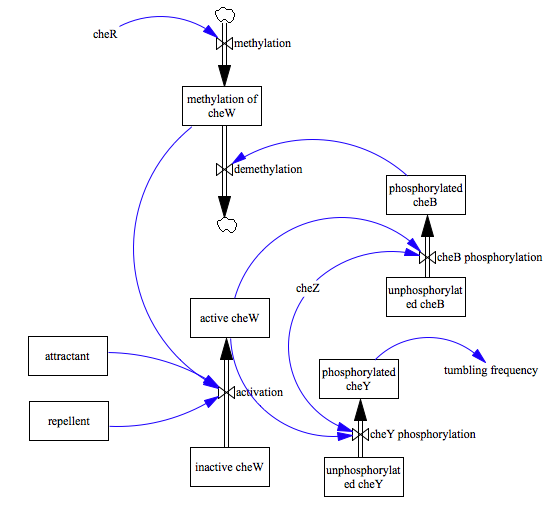
\includegraphics[scale=0.7]{dualstock.png}

The second model approached each active counterpart as a stock, and ignored the inactive versions.  Nothing in the model depended on the quantity of the inactive counterparts anyway, another indication that the dual-stock approach was misguided.  This one was better, but suffered from a chronic tendency to oscillate chaotically out of control.  Once again, a fresh approach was needed.  The main insight I made was to use autoregulation, where the inflow to an active state depended inversely on the amount residing in the stock, and the outflow depended directly on that same amount.  This led to a stable pattern of activity for all the various variables, seeking out a particular level to balance the number flowing in and out of the stock in this way.  No matter what the starting conditions, if left to their own devices all of the stocks would seek out some ideal level.  This idea of autoregulation formed a stable basis for all of the interdependencies between these stocks that would be added later.  

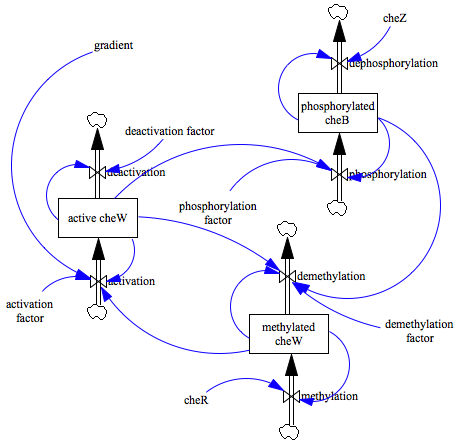
\includegraphics[scale=0.8]{autoregulation.png}

As you can see, the three stocks are active cheW, phosphorylated cheB and methylated cheW.  Active cheW contributes to the phosphorylation of cheB, and cheB joins up with active cheW to contribute to the demethylation of cheW.  Methylated cheW positively influences the activation of cheW.  This is the core loop that was eventually settled on, in addition to supplementary autoregulatory loops between each stock and its respective inflows and outflows.   

\section{Verification}



\section{Validation}



\section{Results}



\section{Learning}

I learned many things above and beyond the basic background for this exercise, many things I did not expect to learn.  One of the big realizations was the value of autoregulation.  \cite{Alon} discusses autoregulation as one of the most basic and most important network motifs.  My earlier



\bibliographystyle{plain}
\bibliography{chemotaxis}

\end{document}